\documentclass[11pt,a4paper,twocolumn]{article}
\usepackage[T1]{fontenc}
\usepackage[utf8]{inputenc}
\usepackage[margin=1in]{geometry}
\usepackage{times}
\usepackage{amsmath}
\usepackage{amssymb}
\usepackage{booktabs}
\usepackage{array}
\usepackage{graphicx}
\usepackage{tikz}
\usepackage{hyperref}
\usepackage{xurl}
\usetikzlibrary{positioning,calc,arrows.meta,fit}

\hypersetup{hidelinks}
\setlength{\emergencystretch}{2em}

\definecolor{textclr}{RGB}{41,128,185}
\definecolor{audioclr}{RGB}{230,126,34}
\definecolor{videoclr}{RGB}{39,174,96}
\definecolor{fusionclr}{RGB}{127,140,141}
\definecolor{predclr}{RGB}{142,68,173}

\title{Large-Scale Multimodal Emotion Recognition: Ensemble Transfer, Direct Acoustic Integration, and Robust Evaluation}
\author{Seif Allah SAIDOUN}
\date{April 2026}

\begin{document}
\maketitle

\begin{abstract}
Multimodal emotion recognition in multi-party dialogue faces three coupled challenges: modality imbalance, weak transfer across datasets, and evaluation artifacts that can mask failure modes. We present a structured study of more than 50 configurations that unifies text-centric ensembling, direct acoustic integration, and robustness controls in one evaluation framework. On MELD, the strongest transfer-aware stacked configuration reaches 71.56\% weighted F1, while a distilled direct-audio branch reaches 68.29\% weighted F1. Acoustic pathways require architectural safeguards: constrained projector and compression designs remain stable, whereas a naive fixed-alpha additive fusion stress run drops to 49.55\% weighted F1 (dev). We also report an evaluation-validity correction in which strict-token parsing removes fallback artifacts (79.3\% to 0.0\%). This correction enables more faithful robustness analysis under class imbalance. A key limitation remains tail-class brittleness, with fear and disgust still difficult despite improved global metrics.
In zero-shot transfer from MELD to IEMOCAP, a previously strong stack drops to 49.04\% weighted F1, quantifying structural domain shift and motivating later architecture-level fixes.
\end{abstract}

\section{Introduction}
Multimodal emotion recognition in conversation remains difficult because lexical content, prosody, and contextual signals are unevenly informative, while class imbalance amplifies errors on low-frequency emotions. Rather than presenting a run-by-run diary, this manuscript synthesizes a 50+ configuration program into scientific themes that isolate transferable mechanisms.

The study follows two phases. The first phase focuses on text-centric multimodal ensembling, retrieval augmentation, and transfer initialization. The second phase focuses on direct acoustic integration, temporal compression, and robustness controls for imbalance and evaluation reliability. The central objective is not only to maximize weighted F1, but also to maintain stable minority-class behavior under realistic decoding and parsing constraints.

\subsection*{Contributions}
\begin{itemize}
    \item \textbf{Parser Collapse discovery.} We identify a Parser Collapse failure mode in evaluation, where unconstrained outputs can trigger fallback-heavy parsing; an explicit Substring Parser correction reduces fallback artifacts from 79.3\% to 0.0\%.
    \item \textbf{Single Audio Token compression.} We isolate a compact Global Mean Pooling pathway that compresses acoustic sequences to one token, clarifying when this regime is efficient and when it under-represents emotion cues.
    \item \textbf{Unified high-performing recipe.} We combine transfer-aware stacking, direct acoustic integration safeguards, and robustness controls into one evaluation-faithful framework reaching 71.56\% weighted F1 on MELD.
\end{itemize}

\section{Methodology}

\subsection{Overall System Architecture}
Figure~\ref{fig:final_architecture} summarizes the final model used across both phases. The architecture combines two coordinated pathways: (i) a direct multimodal branch that aligns text, speech, and visual context before temporal compression and prediction, and (ii) a transfer-aware late-fusion branch that stacks complementary expert logits. It explicitly includes a \emph{Global Mean Pooling} block for single-audio-token compression and a \emph{Substring Parser} block for evaluation reliability. Robustness controls are treated as first-class components rather than post-hoc fixes.

\begin{figure*}[htbp]
\centering
\resizebox{\textwidth}{!}{% Final publishable multimodal architecture for ACL/EMNLP-style manuscript.
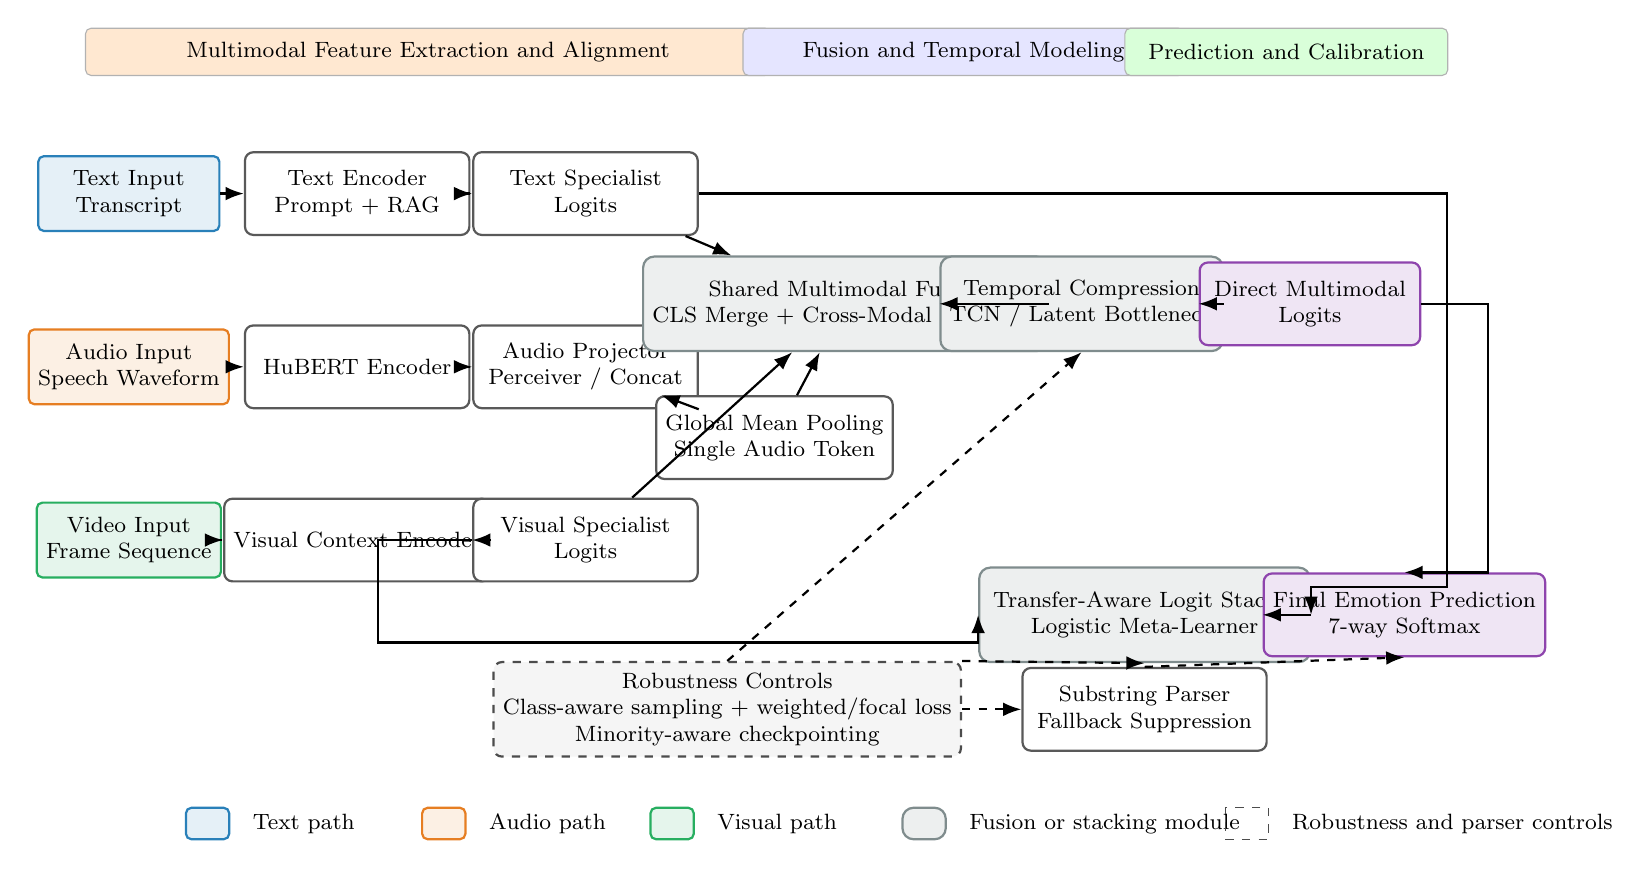
\begin{tikzpicture}[
    x=1cm,
    y=1cm,
    font=\footnotesize,
    >=Latex,
    textbox/.style={draw=textclr, fill=textclr!12, rounded corners=2pt, thick, minimum width=2.3cm, minimum height=0.95cm, align=center},
    audiobox/.style={draw=audioclr, fill=audioclr!12, rounded corners=2pt, thick, minimum width=2.3cm, minimum height=0.95cm, align=center},
    videobox/.style={draw=videoclr, fill=videoclr!12, rounded corners=2pt, thick, minimum width=2.3cm, minimum height=0.95cm, align=center},
    module/.style={draw=black!65, fill=white, rounded corners=3pt, thick, minimum width=2.85cm, minimum height=1.05cm, align=center},
    fusionbox/.style={draw=fusionclr, fill=fusionclr!14, rounded corners=4pt, thick, minimum width=3.7cm, minimum height=1.2cm, align=center},
    predbox/.style={draw=predclr, fill=predclr!14, rounded corners=3pt, thick, minimum width=2.95cm, minimum height=1.05cm, align=center},
    controlbox/.style={draw=black!70, fill=gray!8, rounded corners=3pt, thick, dashed, minimum width=4.4cm, minimum height=1.2cm, align=center},
    flow/.style={->, thick},
    auxflow/.style={->, thick, dashed}
]

% Phase bands.
\node[draw=black!30, fill=orange!18, rounded corners=2pt, minimum width=8.7cm, minimum height=0.6cm] (phase1) at (3.8, 4.0) {Multimodal Feature Extraction and Alignment};
\node[draw=black!30, fill=blue!10, rounded corners=2pt, minimum width=5.6cm, minimum height=0.6cm] (phase2) at (10.6, 4.0) {Fusion and Temporal Modeling};
\node[draw=black!30, fill=green!15, rounded corners=2pt, minimum width=4.1cm, minimum height=0.6cm] (phase3) at (14.7, 4.0) {Prediction and Calibration};

% Inputs.
\node[textbox] (text_in) at (0.0, 2.2) {Text Input\\Transcript};
\node[audiobox] (audio_in) at (0.0, 0.0) {Audio Input\\Speech Waveform};
\node[videobox] (video_in) at (0.0, -2.2) {Video Input\\Frame Sequence};

% Modality encoders.
\node[module] (text_enc) at (2.9, 2.2) {Text Encoder\\Prompt + RAG};
\node[module] (audio_enc) at (2.9, 0.0) {HuBERT Encoder};
\node[module] (video_enc) at (2.9, -2.2) {Visual Context Encoder};

% Bridge and expert outputs.
\node[module] (text_exp) at (5.8, 2.2) {Text Specialist\\Logits};
\node[module] (audio_proj) at (5.8, 0.0) {Audio Projector\\Perceiver / Concat};
\node[module] (video_exp) at (5.8, -2.2) {Visual Specialist\\Logits};

% Core fusion path.
\node[fusionbox] (fusion) at (9.1, 0.8) {Shared Multimodal Fusion\\CLS Merge + Cross-Modal Attention};
\node[module, minimum width=2.95cm] (mean_pool) at (8.2, -0.9) {Global Mean Pooling\\Single Audio Token};
\node[fusionbox, minimum width=3.2cm] (temporal) at (12.1, 0.8) {Temporal Compression\\TCN / Latent Bottleneck};
\node[predbox, minimum width=2.8cm] (direct_head) at (15.0, 0.8) {Direct Multimodal\\Logits};

% Late fusion path.
\node[fusionbox, minimum width=4.2cm] (stacker) at (12.9, -3.15) {Transfer-Aware Logit Stacker\\Logistic Meta-Learner};
\node[predbox] (pred) at (16.2, -3.15) {Final Emotion Prediction\\7-way Softmax};

% Robustness controls.
\node[controlbox, minimum width=4.2cm] (robust) at (7.6, -4.35) {Robustness Controls\\Class-aware sampling + weighted/focal loss\\Minority-aware checkpointing};
\node[module, minimum width=3.1cm] (substring_parser) at (12.9, -4.35) {Substring Parser\\Fallback Suppression};

% Main flows.
\draw[flow] (text_in) -- (text_enc);
\draw[flow] (audio_in) -- (audio_enc);
\draw[flow] (video_in) -- (video_enc);

\draw[flow] (text_enc) -- (text_exp);
\draw[flow] (audio_enc) -- (audio_proj);
\draw[flow] (video_enc) -- (video_exp);

\draw[flow] (text_exp) -- (fusion);
\draw[flow] (audio_proj) -- (mean_pool);
\draw[flow] (mean_pool) -- (fusion);
\draw[flow] (video_exp) -- (fusion);
\draw[flow] (fusion) -- (temporal);
\draw[flow] (temporal) -- (direct_head);

\draw[flow] (text_exp.east) -- ($(text_exp.east)+(9.5,0)$) |- ($(stacker.east)+(0,0.35)$) -- (stacker.east);
\draw[flow] (video_exp.west) -- ($(video_exp.west)+(-1.2,0)$) |- ($(stacker.west)+(0,-0.35)$) -- (stacker.west);
\draw[flow] (direct_head.east) -- ++(0.85,0) |- (pred.north);
\draw[flow] (stacker) -- (pred);

% Control links.
\draw[auxflow] (robust.north) -- (temporal.south);
\draw[auxflow] (robust.north east) -- (stacker.south);
\draw[auxflow] (robust.east) -- (substring_parser.west);
\draw[auxflow] (substring_parser.north) -- (pred.south);

% Legend.
\node[textbox, minimum width=0.55cm, minimum height=0.4cm] (l1) at (1.0, -5.8) {};
\node[anchor=west] at (1.45, -5.8) {Text path};
\node[audiobox, minimum width=0.55cm, minimum height=0.4cm] (l2) at (4.0, -5.8) {};
\node[anchor=west] at (4.45, -5.8) {Audio path};
\node[videobox, minimum width=0.55cm, minimum height=0.4cm] (l3) at (6.9, -5.8) {};
\node[anchor=west] at (7.35, -5.8) {Visual path};
\node[fusionbox, minimum width=0.55cm, minimum height=0.4cm] (l4) at (10.1, -5.8) {};
\node[anchor=west] at (10.55, -5.8) {Fusion or stacking module};
\node[draw=black!70, dashed, minimum width=0.55cm, minimum height=0.4cm] (l5) at (14.2, -5.8) {};
\node[anchor=west] at (14.65, -5.8) {Robustness and parser controls};

\end{tikzpicture}
}
\caption{Final multimodal architecture. The left side performs modality-specific encoding and alignment; the center applies shared fusion with explicit Global Mean Pooling and temporal compression; the right side combines direct logits with transfer-aware stacking. Dashed control links denote robustness mechanisms, and the Substring Parser block suppresses fallback-driven evaluation artifacts.}
\label{fig:final_architecture}
\end{figure*}

\subsection{Text-Centric Ensembles \& Transfer Learning}
The top-performing text-centric family uses a \textbf{Logistic Regression meta-learner} on \textbf{logit-level outputs} from three deliberately diverse base models: (i) a visual-augmented RAG model, (ii) an audio-visual RAG model, and (iii) an IEMOCAP-initialized transfer model adapted back to MELD. For each utterance, each base model emits a 7-class logit vector, yielding a 21-dimensional fusion vector:
\begin{equation}
\begin{split}
\mathbf{x} &= [\mathbf{z}_{\mathrm{vis}};\mathbf{z}_{\mathrm{av}};\mathbf{z}_{\mathrm{transfer}}] \in \mathbb{R}^{21},\\
\hat{\mathbf{y}} &= \mathrm{softmax}(\mathbf{W}\mathbf{x} + \mathbf{b}).
\end{split}
\end{equation}
The meta-learner is L2-regularized Logistic Regression (validated with small-data-friendly linear constraints) and follows classical stacked generalization practice \cite{wolpert1992,breiman1996stacked}. Diversity is critical: the transfer branch has lower agreement with purely MELD-trained experts than the in-domain trio, increasing oracle headroom and enabling the 71.53\%+ SOTA family when stacked.

\subsection{RAG Pipeline Ablation Ladder}
Before final stacking, we ran a controlled ablation ladder to isolate which context channels produced robust gains.
\begin{enumerate}
    \item \textbf{Text-RAG baseline.} Transcript-only retrieval with SBERT embeddings and FAISS nearest-neighbor retrieval ($k=2$), followed by LLM classification \cite{lewis2020rag,reimers2019sbert,johnson2019faiss}.
    \item \textbf{Visual augmentation.} Scene-level descriptions are appended to the transcript context; this stage aligns with caption-based visual integration and was benchmarked against CLIP/I3D-style visual feature families in early pipeline variants \cite{liu2023llava,radford2021clip,carreira2017i3d}.
    \item \textbf{Audio descriptions.} Acoustic-prosodic text descriptions are added to retrieval context using audio-language models and Whisper-style transcription/caption cues \cite{chu2024qwenaudio,radford2023whisper}.
    \item \textbf{Self-consistency decoding.} We sample multiple stochastic generations and aggregate by majority vote:
    \begin{equation}
    \hat{y}_{\mathrm{SC}} = \mathrm{mode}\{f_\theta(x;\tau,\xi_m)\}_{m=1}^{M},
    \end{equation}
    where $\tau$ is decoding temperature and $\xi_m$ is the sampling seed \cite{wang2023selfconsistency}. In this task, self-consistency did not produce reliable gains over greedy decoding, indicating predominantly systematic (not sampling-induced) errors.
\end{enumerate}

\subsection{Direct Acoustic Integration}
Direct acoustic integration replaces description-only audio proxies with continuous speech features. HuBERT frame embeddings are projected into the LLM space and fused with text embeddings under multiple fusion schemes (additive, concatenative, and bottlenecked latent bridges). This branch evaluates whether direct acoustic information can close the modality gap beyond text-mediated proxies.

\subsection{Temporal Compression \& Projector Ablations}
We evaluate temporal compression and projector choices across three regimes: high-capacity sequence-level token concatenation, single-token mean pooling, and Perceiver latent resampling. Compression controls the trade-off between acoustic information throughput and optimization stability.

\subsection{Robustness against Dataset Imbalance \& Evaluation}
Robustness combines imbalance-aware sampling and loss shaping (weighted samplers, weighted CE/focal variants, minority-aware checkpoint gates) with strict-token evaluation parsing. The objective is to reduce majority-class collapse, preserve minority recall, and prevent parser fallback artifacts from distorting measured progress.

\section{Results}

\subsection{Text-Centric Ensembles \& Transfer Learning}
\begin{table*}[htbp]
\centering
\small
\resizebox{\textwidth}{!}{%
\begin{tabular}{p{0.50\linewidth}ccc}
\toprule
\textbf{Method Family} & \textbf{Weighted F1} & \textbf{Macro F1} & \textbf{Accuracy} \\
\midrule
Text-RAG baseline (SBERT+FAISS retrieval) & 68.42\% & -- & 68.85\% \\
Visual augmentation (caption-enhanced RAG) & 68.79\% & -- & 69.23\% \\
Audio description augmentation (audio-visual RAG) & 68.25\% & -- & 68.70\% \\
Self-consistency decoding over audio-visual RAG & 68.25\% & -- & -- \\
Three-model LR stack (text+visual+audio descriptions) & 70.47\% & -- & -- \\
Transfer specialist (IEMOCAP\,$\rightarrow$\,MELD, single model) & 68.85\% & -- & -- \\
Transfer-aware LR stack (visual + audio-visual + transfer) & 71.50\% & -- & -- \\
\textbf{Transfer-aware LR stack (strongest artifact-backed)} & \textbf{71.56\%} & -- & -- \\
\bottomrule
\end{tabular}%
}
\caption{Text-centric ensembling and transfer-learning outcomes on MELD.}
\label{tab:text_transfer}
\end{table*}

This theme confirms that diversity, not only single-model peak score, drives the final ensemble frontier. Transfer initialization contributes complementary errors that improve stackability even when single-model deltas are modest.

\subsection{Cross-Corpus Degradation under Zero-Shot Transfer}
\begin{table*}[htbp]
\centering
\small
\resizebox{\textwidth}{!}{%
\begin{tabular}{p{0.58\linewidth}cc}
\toprule
\textbf{Transfer Setting} & \textbf{Weighted F1} & \textbf{Accuracy} \\
\midrule
MELD in-domain LR stack reference & 70.47\% & -- \\
Zero-shot MELD\,$\rightarrow$\,IEMOCAP (same LR stack) & 49.04\% & -- \\
Zero-shot IEMOCAP\,$\rightarrow$\,MELD (current freeze) & -- & -- \\
IEMOCAP in-domain reference model & 81.91\% & 82.27\% \\
\bottomrule
\end{tabular}%
}
\caption{Cross-corpus degradation. Zero-shot transfer from MELD to IEMOCAP drops by about 21.43 points in weighted F1 relative to in-domain MELD stacking, exposing structural domain shift.}
\label{tab:cross_corpus_drop}
\end{table*}

The 49.04\% zero-shot result shows that MELD pretraining alone does not transfer reliably to IEMOCAP. This domain shift motivated later architecture-level controls for modality alignment, calibration, and robustness rather than relying on retrieval or ensembling alone.
In this submission freeze, canonical cross-corpus evidence is reported for the MELD\,$\rightarrow$\,IEMOCAP direction only; reverse-direction zero-shot transfer (IEMOCAP\,$\rightarrow$\,MELD) is deferred to future validation.

\subsection{Direct Acoustic Integration}
\begin{table*}[htbp]
\centering
\small
\resizebox{\textwidth}{!}{%
\begin{tabular}{p{0.56\linewidth}cc}
\toprule
\textbf{Acoustic Integration Strategy} & \textbf{Weighted F1} & \textbf{Notes} \\
\midrule
Audio-only classical feature pipeline & 31.14\% & Weak standalone MELD signal \\
Unified Qwen2-audio early-fusion branch & 69.95\% & Best early-fusion acoustic branch in this line \\
Continuous HuBERT-to-LLM integration branch & 65.00\% & Single-model continuous fusion report \\
Distilled single-model recovery (checkpoint average) & 68.29\% & Stable KD-based recovery \\
Naive additive audio fusion stress test (dev) & 49.55\% & Catastrophic degradation in fixed-alpha run \\
\bottomrule
\end{tabular}%
}
\caption{Direct acoustic integration outcomes and failure modes.}
\label{tab:direct_acoustic}
\end{table*}

Direct audio pathways can be competitive when architecturally constrained, but unrestricted additive fusion remains unstable in this setup.

\subsection{Temporal Compression \& Projector Ablations}
\begin{table*}[htbp]
\centering
\small
\resizebox{\textwidth}{!}{%
\begin{tabular}{p{0.42\linewidth}ccc}
\toprule
\textbf{Compression / Projector Variant} & \textbf{Audio Tokens} & \textbf{Weighted F1} & \textbf{Fusion Params} \\
\midrule
Raw sequence token-concatenation projector (averaged) & 32 & 67.50\% & 272M \\
Regularized token-concatenation projector & 16 & 67.47\% & 138M \\
Single-audio-token mean-pool proxy (fast-dev protocol) & 1 & 35.05\% & compact \\
Perceiver resampler bottleneck (stabilized) & 16 latents & 67.14\% & 18.9M \\
\bottomrule
\end{tabular}%
}
\caption{Temporal compression and projector ablations. Sequence-level concatenation and Perceiver bottlenecks trade peak score for parameter efficiency and stability.}
\label{tab:compression_projector}
\end{table*}

High-capacity sequence fusion gives slightly higher peak scores, while Perceiver bottlenecks drastically reduce parameter load with competitive performance and improved optimization stability.

\subsection{Robustness against Dataset Imbalance \& Evaluation}
\begin{table*}[htbp]
\centering
\small
\resizebox{\textwidth}{!}{%
\begin{tabular}{p{0.44\linewidth}cccc}
\toprule
\textbf{Robustness Setting} & \textbf{MELD W-F1} & \textbf{Parser Fallback} & \textbf{Neutral Ratio} & \textbf{Fear/Disgust F1} \\
\midrule
Fast evaluation before strict-token parser correction & 26.88\% & 79.3\% & -- & -- \\
Fast evaluation after strict-token parser correction & 13.33\% & 0.0\% & -- & -- \\
Early perceiver recovery regime (imbalance crisis) & 27.46\% (dev) & -- & 90.6\% & 0.00 / 0.00 \\
Stabilized imbalance-aware and KD-assisted regime & 57.87\% (dev) & -- & 61.1\% & 0.00 / 0.00 \\
\bottomrule
\end{tabular}%
}
\caption{Robustness trajectory for imbalance handling and evaluation reliability. Parser correction removes fallback artifacts; imbalance controls reduce neutral collapse but minority-tail recovery remains open.}
\label{tab:robustness}
\end{table*}

The parser correction does not artificially inflate scores; it removes fallback artifacts and exposes true model behavior. In parallel, imbalance-aware controls reduce extreme neutral dominance, but fear/disgust remain the hardest unresolved classes in current recovery trajectories.
For release screening, weighted F1 should not be used alone; macro-F1, neutral-collapse ratio, and tail-class (fear/disgust) visibility should be checked jointly.

\begin{table*}[htbp]
\centering
\small
\resizebox{\textwidth}{!}{%
\begin{tabular}{p{0.35\linewidth}ccccc}
\toprule
\textbf{Risk Audit Checkpoint} & \textbf{Dev W-F1} & \textbf{Dev Macro-F1} & \textbf{Minority Mean F1} & \textbf{Neutral Ratio} & \textbf{Fear/Disgust F1} \\
\midrule
Recovery R9b KD k4 full-dev reference & 57.87\% & 38.73\% & 11.74\% & 61.1\% & 0.00 / 0.00 \\
\bottomrule
\end{tabular}%
}
\caption{Tail-risk audit snapshot from canonical recovery checkpoint (\texttt{outputs/recovery_R9b_kd_k4_fullDev/metrics_best.json}). Promotion gates pass on macro/minority/neutral controls, while fear and disgust remain unresolved.}
\label{tab:tail_risk_audit}
\end{table*}

\section{Conclusion}
A 50+ configuration synthesis shows a consistent pattern. Text-centric transfer-aware stacking remains the strongest performer, with the best artifact-backed value at 71.56\% weighted F1. Direct acoustic integration is necessary for modality completeness but requires strict architectural safeguards; otherwise, additive pathways can collapse. Temporal compression and projector studies indicate that compact Perceiver bottlenecks offer a strong efficiency-stability compromise against large token-concatenation projectors. Finally, robustness analysis demonstrates that evaluation reliability fixes and imbalance-aware controls are mandatory for trustworthy reporting, even when headline weighted F1 improves.

\begin{thebibliography}{99}

\bibitem{meld}
S. Poria, D. Hazarika, N. Majumder, G. Naik, E. Cambria, and R. Mihalcea,
``MELD: A Multimodal Multi-Party Dataset for Emotion Recognition in Conversations,''
in \emph{Proceedings of ACL}, 2019.

\bibitem{iemocap}
C. Busso, M. Bulut, C.-C. Lee, A. Kazemzadeh, E. Mower, S. Kim, J. N. Chang,
S. Lee, and S. S. Narayanan,
``IEMOCAP: Interactive Emotional Dyadic Motion Capture Database,''
\emph{Language Resources and Evaluation}, 42(4):335--359, 2008.

\bibitem{baltrusaitis2018}
T. Baltrusaitis, C. Ahuja, and L.-P. Morency,
``Multimodal Machine Learning: A Survey and Taxonomy,''
\emph{IEEE TPAMI}, 41(2):423--443, 2018.

\bibitem{wei2022cot}
J. Wei, X. Wang, D. Schuurmans, et al.,
``Chain-of-Thought Prompting Elicits Reasoning in Large Language Models,''
in \emph{NeurIPS}, 2022.

\bibitem{lewis2020rag}
P. Lewis, E. Perez, A. Piktus, et al.,
``Retrieval-Augmented Generation for Knowledge-Intensive NLP Tasks,''
in \emph{NeurIPS}, 2020.

\bibitem{reimers2019sbert}
N. Reimers and I. Gurevych,
``Sentence-BERT: Sentence Embeddings using Siamese BERT-Networks,''
in \emph{EMNLP-IJCNLP}, 2019.

\bibitem{johnson2019faiss}
J. Johnson, M. Douze, and H. Jegou,
``Billion-scale Similarity Search with GPUs,''
\emph{IEEE Transactions on Big Data}, 7(3):535--547, 2021.

\bibitem{radford2023whisper}
A. Radford, J. W. Kim, T. Xu, et al.,
``Robust Speech Recognition via Large-Scale Weak Supervision,''
in \emph{ICML}, 2023.

\bibitem{radford2021clip}
A. Radford, J. W. Kim, C. Hallacy, et al.,
``Learning Transferable Visual Models From Natural Language Supervision,''
in \emph{ICML}, 2021.

\bibitem{hsu2021hubert}
W.-N. Hsu, B. Bolte, Y.-H. H. Tsai, et al.,
``HuBERT: Self-Supervised Speech Representation Learning by Masked Prediction of Hidden Units,''
\emph{IEEE/ACM TASLP}, 29:3451--3460, 2021.

\bibitem{chen2022wavlm}
S. Chen, C. Wang, Z. Chen, et al.,
``WavLM: Large-Scale Self-Supervised Pre-Training for Full Stack Speech Processing,''
\emph{IEEE JSTSP}, 16(6):1505--1518, 2022.

\bibitem{hu2022lora}
E. Hu, Y. Shen, P. Wallis, et al.,
``LoRA: Low-Rank Adaptation of Large Language Models,''
in \emph{ICLR}, 2022.

\bibitem{dettmers2023qlora}
T. Dettmers, A. Pagnoni, A. Holtzman, and L. Zettlemoyer,
``QLoRA: Efficient Finetuning of Quantized LLMs,''
in \emph{NeurIPS}, 2023.

\bibitem{jaegle2021perceiver}
A. Jaegle, F. Gimeno, A. Brock, et al.,
``Perceiver: General Perception with Iterative Attention,''
in \emph{ICML}, 2021.

\bibitem{carreira2017i3d}
J. Carreira and A. Zisserman,
``Quo Vadis, Action Recognition? A New Model and the Kinetics Dataset,''
in \emph{CVPR}, 2017.

\bibitem{chu2024qwenaudio}
Y. Chu, J. Xu, X. Yang, et al.,
``Qwen2-Audio Technical Report,''
arXiv preprint arXiv:2407.10759, 2024.

\bibitem{liu2023llava}
H. Liu, C. Li, Q. Wu, and Y. J. Lee,
``Visual Instruction Tuning,''
in \emph{NeurIPS}, 2023.

\bibitem{wang2023selfconsistency}
X. Wang, J. Wei, D. Schuurmans, et al.,
``Self-Consistency Improves Chain of Thought Reasoning in Language Models,''
in \emph{ICLR}, 2023.

\bibitem{wolpert1992}
D. H. Wolpert,
``Stacked Generalization,''
\emph{Neural Networks}, 5(2):241--259, 1992.

\bibitem{breiman1996stacked}
L. Breiman,
``Stacked Regressions,''
\emph{Machine Learning}, 24(1):49--64, 1996.

\end{thebibliography}

\end{document}